\documentclass[conference]{IEEEtran}

\usepackage{svg}


\hyphenation{op-tical net-works semi-conduc-tor}

% Document.
\begin{document}

\title{Comparative analysis of performance using server-client protocols}

\author{\IEEEauthorblockN{Mihail Costea}
\IEEEauthorblockA{University Politehnica of Bucharest\\
The Faculty of Automatic Control and Computers\\
Bucharest, Romania\\
Email: mihail.costea90@gmail.com}
\and
\IEEEauthorblockN{Liviu Chircu}
\IEEEauthorblockA{University Politehnica of Bucharest\\
The Faculty of Automatic Control and Computers\\
Bucharest, Romania\\
Email: liviu.chircu@gmail.com}}

\maketitle

\begin{abstract}
TODO - add references
\\
\indent
Current web applications' solutions for bi-directional communication are based on AJAX.
Even though they are well documented solutions that are backed up by years of
utilization, they have limitations imposed by the HTTP protocol. HTTP is a
stateless protocol that requires each connection to be treated as a new
connection, requiring unnecessary overhead to communicate in both directions.
Because of these limitations a new solution was developed, WebSockets,
which are able to natively mantain a bi-directional channel, reducing the
overhead needed for communication.
\\
\indent
This paper proposes to exemplify the advantages and disadvantages between
traditional HTTP implementations for bi-directional communication based on AJAX
and WebSockets. Also it proposes an architecture for a testing platform for
different WebSockets implementations.
\end{abstract}

\IEEEpeerreviewmaketitle

% Content.
\section{Introduction}
After the introduction of Web 2.0, web applications are able to modify the
content of HTML documents without refresh, offering better interactive to end-user.
The most popular technology used for creating this interactivity is AJAX
(Asynchronous JavaScript and XML). This way pages can be updated in real-time,
without needing an explicit action from the user. But because AJAX is based on
HTTP, a stateless protocol that requires each connection to be treated as a new
connection, creating bi-directional channels between 2 devices imposes unnecessary
overhead, as both nodes need to mimic this channel that require states.
Bi-directional channels are necessary for web applications, like chat, games,
video calls, where a lot of data is transmitted in both directions.
\\
\indent
The most popular solutions used by AJAX are: polling, where a client sends
a request to a server at regular intervals and the server responses immediately
and closes the connection; long-polling, where the client sends a request to the
server as soon as it receives any data from the server, and the server keep that
connection open until it has data to send to the client; streaming, where the
connection between client and server is kept alive indefinitely and data is streamed,
until one of them closes the connection. The problem with last solution is that AJAX
appends the new data to previously sent data until the connection end, which is
unnecessary in many cases. Also HTTP headers must be send whenever a new connection is
created, which is a common case for polling and long-polling. If a lot of small data
is sent, as in the case of chat application, this overhead might be to much compared
to the data (\textbf{add reference in bibliography \cite{1}}).
\\
\indent
In order to overcome to limitations of AJAX based solutions, WebSockets were created.
This is a new technology based on HTTP (\textbf{add RFC reference in bibliography \cite{2}}).
HTTP was chosen as a base because most firewalls allow HTTP and HTTPS traffic 
(ports 80 and 443), while other ports' traffic might be blocked. Though it's based on
HTTP, it doesn't inherit its limitations. HTTP is used only for creating and
closing the connection between client and server, and not the connection itself.
The distinction between normal HTTP traffic and WebSockets is done through the
"Upgrade: websocket"/"Connection: Upgrade" headers (\textbf{RFC reference \cite{2}}).
\\
\indent
Just as mentioned above, Websockets is a new technology created recently
(the RFC was written in 2011), so it isn't very well tested. This can be
considered one of the minuses compared to AJAX, which is better tested.
There have been created testing platforms for the validations of WebSockets
implementations, in order to make sure they work correctly
(\textbf{give a few examples}), but, to our best knowledge, there aren't any
testing platforms for the performance of WebSockets implementations.
This paper compares AJAX with WebSockets and proposes an architecture for
a testing platform, which should be independent of Operating System and devices.
It should work for both laptops and smartphones, for Windows and Linux and
other devices and Operating Systems.

\section{Related work}
\textit{Real-time Monitoring using AJAX and WebSockets} paper (\textbf{create reference})
exemplifies the differences in terms of performance between AJAX and WebSockets.
The authors added real-time monitoring support for OASIS (\textbf{maybe reference}),
an open-source real-time instrumentation middleware for distributed real-time
and embedded systems. The collected instrumentation data was sent over the Web
using AJAX and WebSockets and the results were compared. The WebSockets server
consumes 50% less network bandwidth then the AJAX server. Also the WebSockets
client consumes memory at a constant rate, while the AJAX client consumes it
at an increasing rate and Websockets can send up to 215.44% more data sample
than AJAX by using the same amount of network bandwidth.
\\
\begin{frame}{}
  \begin{figure}
    \centering
    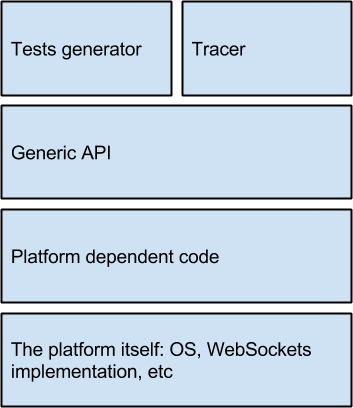
\includegraphics[width=0.4\textwidth]{Architecture.png}
    \caption{Performance application architecture}
  \end{figure}
\end{frame}
\indent
Another example where WebSockets are better than AJAX is the case of sending
small data per frame. When WebSockets exchange 2B of data per frame, continuous
polling with AJAX exchange up to 8 KB of HTTP header (\textbf{create reference}).
\\
\indent
Even though WebSockets are better than AJAX based solutions, it's still not as
good as raw TCP sockets. \textit{Real-time Web Application Roadblock:
Performance Penalty of HTML Sockets} paper (\textbf{create reference}) discusses
the penalties of using HTML socket streams (long-polling and WebSockets)
vs TCP streams. HTML socket streams can have up to 5x protocol overhead, up to
3x more payload delivery delay and up to 3x less throughput. In case of small
data payload (a few hundreds of bytes), the performance between the 2 is
pretty high. Also TCP streams a behave better over 3G than HTML socket streams.
One reason for the poorer performance is given by the fact that the browser uses
buffering for HTML socket streams (both long-polling and WebSockets), introducing
delays, while TCP sockets cand send the data directly. But on the good side for
WebSockets, the paper mentions that they behave better than long-polling when
it comes to sending small-size chunks, making it a better choice for chat,
voip, online games, etc, just like TCP streams. As a big plus for HTML sockets
compared to TCP streams is the fact that the data send with them can pass over
firewalls and most proxies, as HTTP and HTTPS are usually not blocked.

\section{Architecture}
This section proposes a simple architecture for an application that must test
the performance of WebSockets and AJAX implementations of bi-directional
communication. Figure 1 contains the architecture and the layers. In order to
test the performance automatically, the application should be able to generate
tests based on a given input and automatically measure how those tests behave
on a given platform. The design should promote easy porting to other devices
and Operating Systems. It should have a layer independent of the platform and
of the implementation of either WebSockets or AJAX. The layer provides a generic
API that is used by the tests generator component and the tracer or measurements
component. The API and the previously mentioned components are going to be ported
to other platforms with minimal changes. The layer that provides the API is going
to be implemented by every platform in a different ways that depends on the
Operating System, how the WebSockets API looks, etc.

\bibliography{bare_conf}{}
\bibliographystyle{unsrt}

\end{document}


